\documentclass[]{article}
\usepackage[utf8]{inputenc}
\usepackage[croatian]{babel}
\usepackage{graphicx}
\usepackage{enumerate}


%opening
\title{Web galerija za višemedijske sustave}
\author{Tina Marić, Gregor Boris Banušić}

\begin{document}

\maketitle


\section{Uvod}
Web galerija je web stanica napravljena u svrhu organiziranja materijala sa kolegija "Višemedijski sustavi".
Ideja je u galeriju pohraniti sve slike, video sadržaje, projekte i prezentacije na jednom mjestu tako da budu dohvatljive svim studentima koji su zainteresirani za kolegij.
\newline
\newline
\subsection{Implementacija}
\textbf{Backend} je implementiran pomoću sljedećih tehnologija:
\begin{itemize}
	\item ruby on rails (RoR),
\end{itemize}
dok je za \textbf{frontend} korišteno:
\begin{itemize}
	\item Bootstrap (Pingendo program),
	\item HTML,
	\item CSS,
	\item Javascript.
\end{itemize}

Trenutnu verziju možete vidjeti na:

\textbf{https://ancient-fortress-78196.herokuapp.com/}

\newpage

\subsection{Struktura koda}
Za unaprjeđivanje projekta koristit će se većinom datoteke označene u narednoj slici. U folderu "assets" se nalaze slike koje koristimo za izgled web stranice ("hardkodirane slike").

\begin{figure}[h]
	\centering
	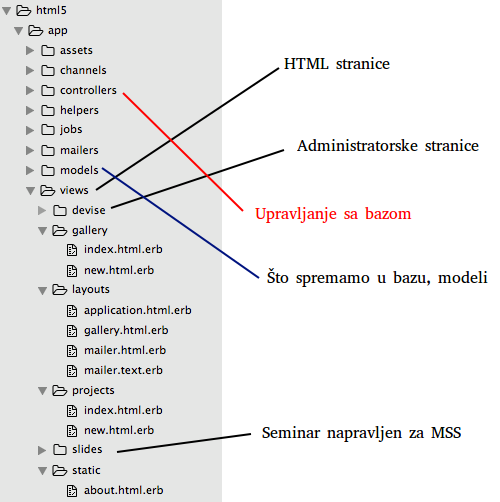
\includegraphics[scale=0.5]{struktura-projekta}
	\caption{Struktura projekta}
	\label{fig:mesh1}
\end{figure}

Nedostatci:
\begin{itemize}
	\item dokumentacija gdje se što nalazi
	\item treba poznavati dobro RoR alat
\end{itemize}
\newpage


\section{Dizajn web galerije}

Galerija se sastoji od više stranica (linkova) koje zajedno čine cjelinu.
Sve stranice nalaze se u navigacijskom izborniku na vrhu stranice. Navigacijski izbornik bi se trebao sastojati od linkova za:

\begin{itemize}
	\item Galerija slika
	\item Video galerija*
	\item Audio zapisi*
	\item O kolegiju (pravila kolegija)
	\item Projekti
\end{itemize}

\begin{footnotesize}
	(* nije implementirano)
\end{footnotesize}
\\
\\
\\
\begin{figure}[h]
	\centering
	
\includegraphics[scale=0.5]{nav-bar}
	\caption{Navigacijski izbornik( bez Video i Audio)}
	\label{fig:mesh1}
\end{figure}

Nedostatci:
\begin{itemize}
	\item navigacijski izbornik ne radi za male ekrane (kad se smanji dobije se gumb koji ne radi na klik u google chrome-u) 
\end{itemize}

\newpage
\subsection{Galerija}
\textit{Galerija slika} sadrži sve slike koje su stavljene na server od strane administratora.
(Više o stavljanju slika na server kasnije.)
\\
\begin{figure}[h]
	\centering
	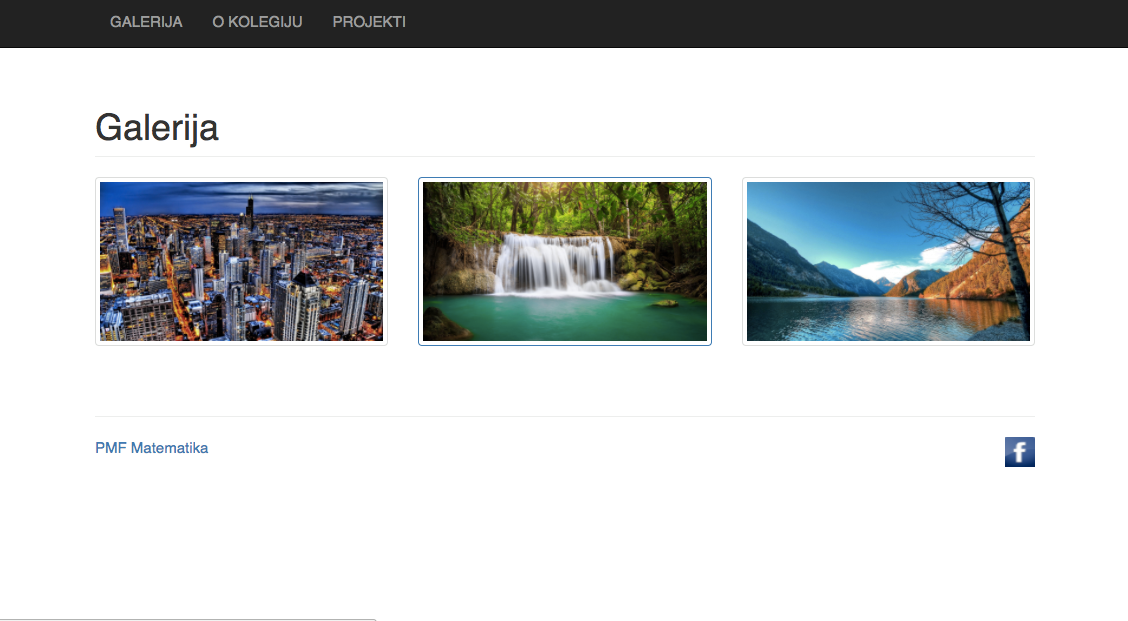
\includegraphics[scale=0.23]{galerija}
	\caption{Galerija slika}
	\label{fig:mesh1}
\end{figure}

Također sadrži takozvani "slider" tj. prikaz slika nakon klika na njih. Pomoću gumbova se može kretati po galeriji lijevo odnosno desno ili izaći iz prikaza slika. Svaka slika ima svoje ime koje se prikazuje nakon klika. Slike su sortirane po datumu kada su stavljene (od najnovije prema starijima).
\\
\begin{figure}[h]
	\centering
	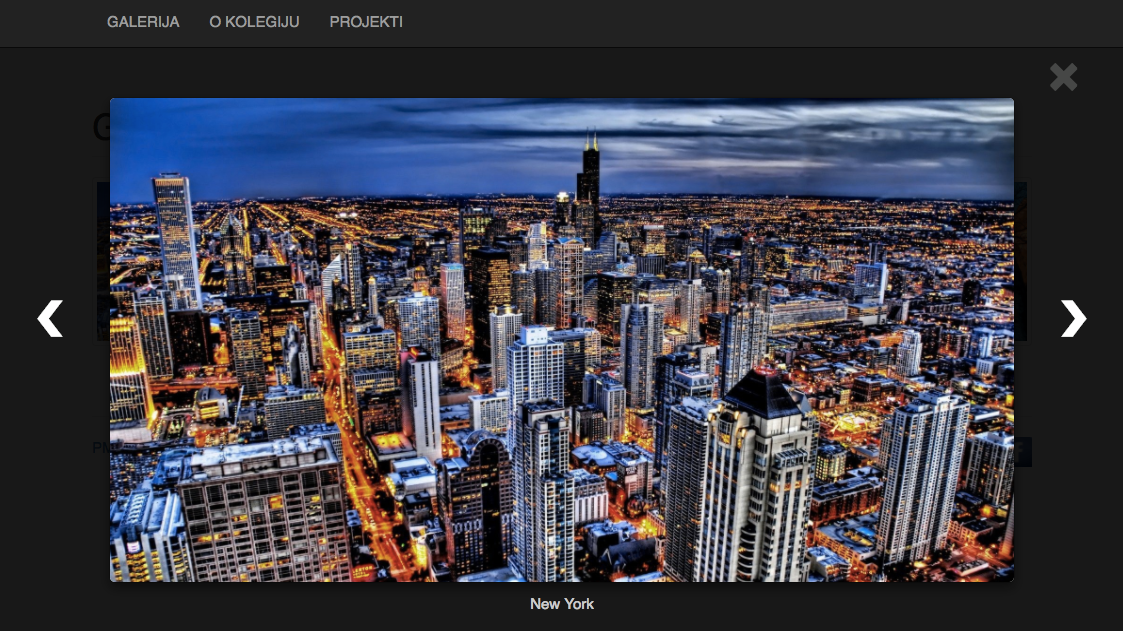
\includegraphics[scale=0.23]{slider}
	\caption{Slider}
	\label{fig:mesh1}
\end{figure}

Nedostatci:
\begin{itemize}
	\item filtriranja/pretraživanja po tematici
	\item kategorizacija slika
	\item pojedine slike su premale pa je prikaz u galeriji loš, prilagoditi prikaz velicini slike
\end{itemize}
\newpage
\subsection{Video*}
Stranica video galerija bi trebala sadržavati niz videa sortiranih po datumu kada su stavljeni na server. Po videima bi se također moglo kretati lijevo odnosno desno kao u galeriji slika.
\\
\\
Implementirati:
\begin{itemize}
	\item prikaz slika iz videa
	\item klikom na video se prikaže modal koji izvodi video
	\item možemo se kretati po videima lijevo odnosno desno, izlazi se pritiskom na gumb \textbf{X}
	\item spremati podatke o videu u bazu podataka (backend)
\end{itemize}

\subsection{Audio*}
Audio stranica bi sadržavala samo jedan "audio" tag koji bi izvodio pjesmu ovisno o kliknutoj pjesmi iz albuma, koji bi se nalazio ispod. Slika u nastavku prikazuje izgled audio stranice.
\\
\\
Implementirati:
\begin{itemize}
	\item izabrati sliku koja će se prikazivati za svaki audio zapis
	\item audio zapisi se trebaju prikazivati sa imenom audia
	\item automatski klikom na audio zapis se prebacuje pjesma i odmah izvodi
	\item spremati podatke audia u bazu podataka (backend)
\end{itemize}

\begin{figure}[h]
	\centering
	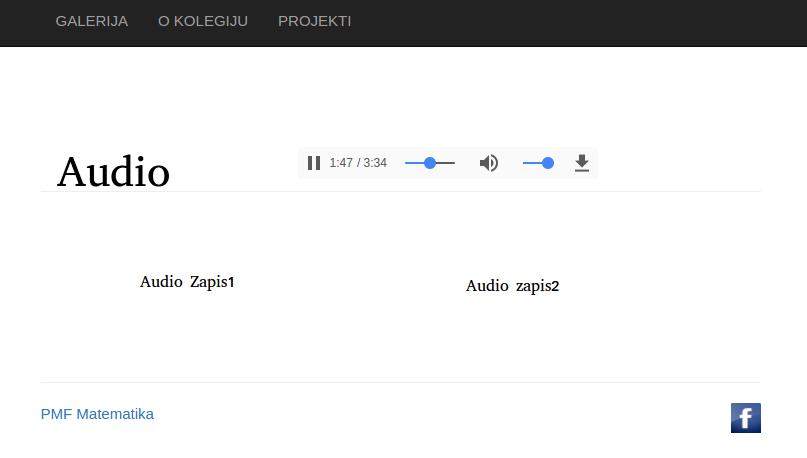
\includegraphics[scale=0.3]{audio}
	\caption{Audio stranica}
	\label{fig:mesh1}
\end{figure}

\newpage

\subsection{Administratorske ovlasti}
Dodatno, za administratore web stranice imamo posebne linkove:
\begin{itemize}
	\item "$^{*2}$/admins/sign\_up" za stvaranje administratora
	\item "$^{*2}$/admins/sign\_in" za login sa administratorom
\end{itemize}

\begin{footnotesize}
	($^{*2}$trenutno: https://ancient-fortress-78196.herokuapp.com/)
\end{footnotesize}
\\
\\
Nakon login-a sa računom administratora dobivamo nova dva taba "Dodaj sliku" i "Odjava" te još neke funkcionalnosti. Dodaj sliku implementira funkcionalnosti za dodavanje slike u galeriju te dodjeljivanje imena uploudanoj slici. U galeriji se pojavi link za brisanje svake stavljene slike. Također, na linku projekti se mogu dodavati te brisati novi linkovi na projekte studenata koji su svoj rad objavili na internetu.
\\
\\
\begin{figure}[h]
	\centering
	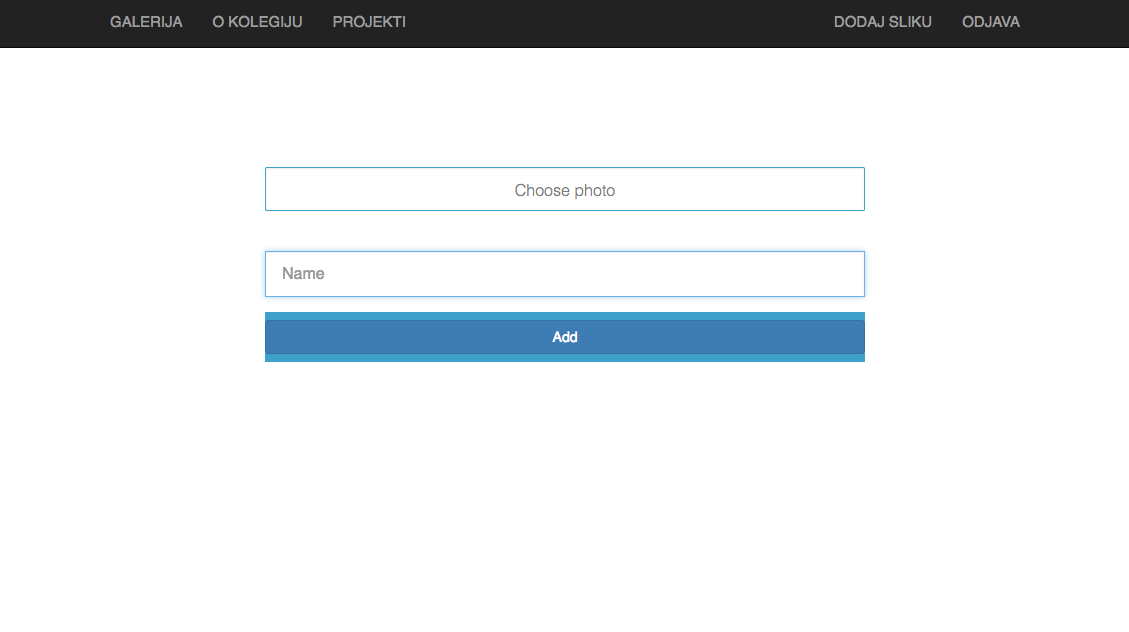
\includegraphics[scale=0.22]{dodaj-sliku}
	\caption{Dodavanje slika kao administratora}
	\label{fig:mesh1}
\end{figure}

\begin{figure}[h]
	\centering
	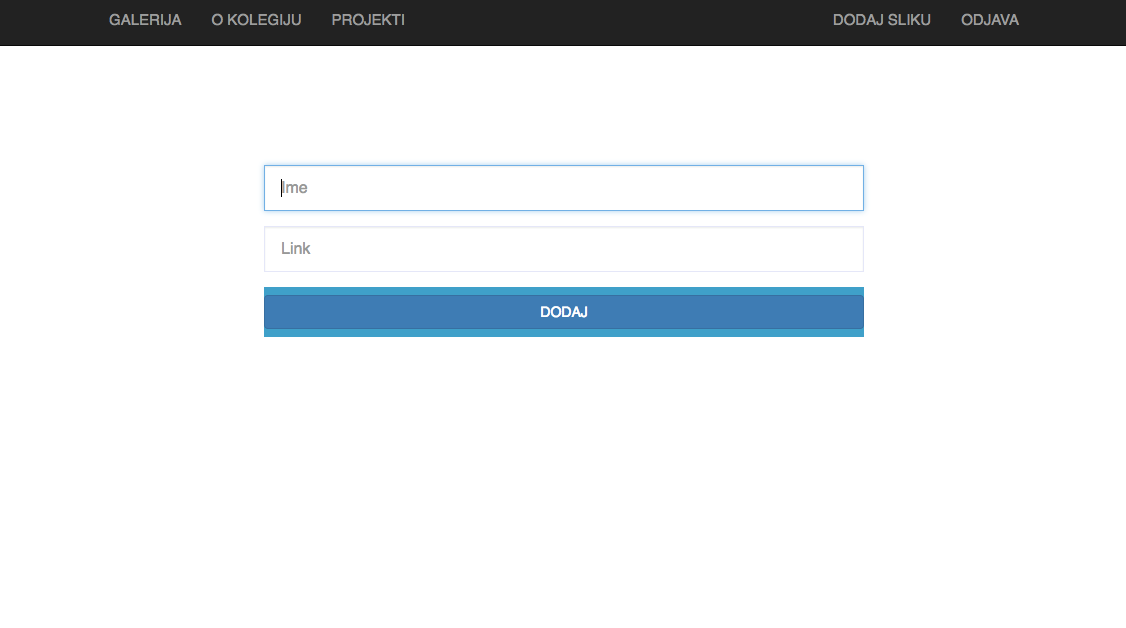
\includegraphics[scale=0.22]{dodaj-projekt}
	\caption{Dodavanje link-a na projekt kao administratora}
	\label{fig:mesh1}
\end{figure}

\newpage

Nedostatci:
\begin{itemize}
	\item dodavanje videa
	\item dodavanje audia
	\item prebacivanje funkcionalnosti "dodaj sliku" na stranicu gdje je galerija
	\item \textbf{forma se može ispunjavati samo pomoću taba trenutno (problem sa css-om pretpostavljamo)}
	\item promjena o kolegiju stranice nije moguća osim ručno u "static/about.html.erb" file-u
\end{itemize}
\newpage
\subsection{O kolegiju}
Stranica o kolegiju prikazuje podatke o kolegiju tj. o Višemedijskim sustavima.
\\
\\
\begin{figure}[h]
	\centering
	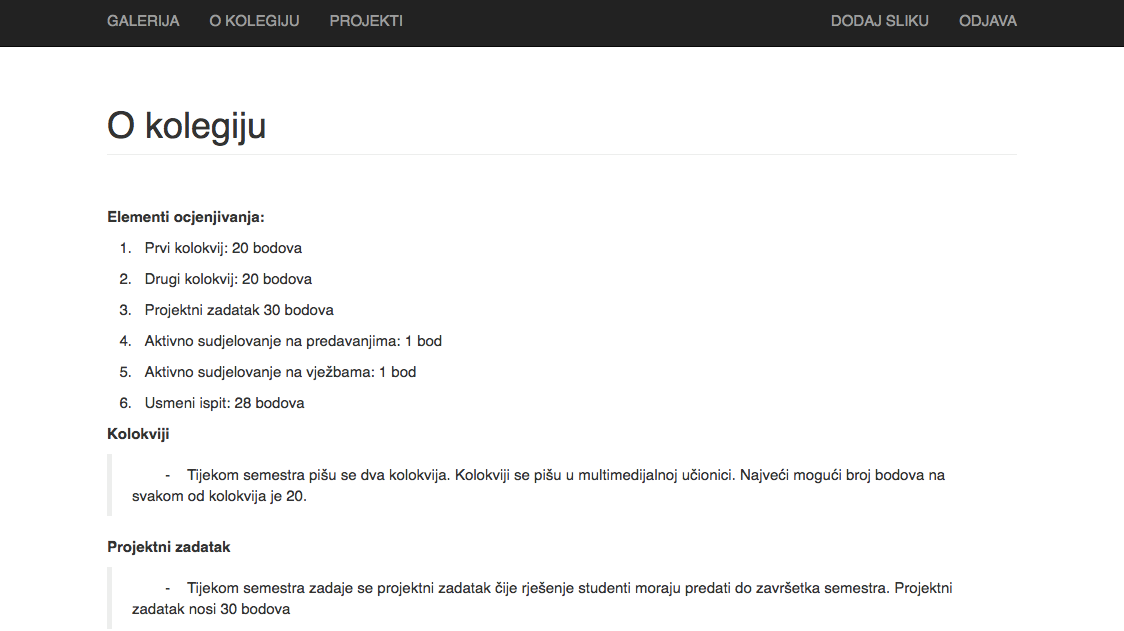
\includegraphics[scale=0.22]{o-kolegiju}
	\caption{O kolegiju sadržaj}
	\label{fig:mesh1}
\end{figure}


\end{document}
